\documentclass{beamer}
\usepackage{amsmath}
\usepackage{graphicx}
\mode<presentation>
{
  \usetheme{default}
  \usecolortheme{seahorse}
}

\title{Formal Verification of Moonshot SMR Protocol}
\author{Saurabh Joshi, Isaac Doidge, Raghavendra Ramesh, Nibesh
Shrestha\textbar Chandradeep Dey, Gangamreddypalli Namratha Reddy, M.~Praveen}
\institute{Supra Oracles \textbar~ Chennai Mathematical Institute}
\date{November 2023}

\begin{document}
\begin{frame}
    \titlepage
\end{frame}

\begin{frame}
    \frametitle{Goal of the Project}
    \begin{itemize}
        \item The Moonshot State Machine Replication protocol has been
            proven to be safe and live by the Supra Research team
            \pause
            \vfill
        \item The goal of this project is to write the above safety
            proof in a formal logical language and verify its
            correctness
            \pause
            \vfill
        \item What is gained from this exercise? \pause
            \vfill
            \begin{itemize}
                \item Confidence that there are no errors in the proof
                    \pause
                    \vfill
                \item Possibility of generating test cases from the
                    formal proof constructed
            \end{itemize}
    \end{itemize}
\end{frame}

\begin{frame}
    \frametitle{Tools and Methods Used}
    \begin{itemize}
        \item \alert{IVy}: a deductive
            verification tool, verified Tendermint, HotStuff etc.
            \pause
            \vfill
        \item Moonshot pseudocode $\Rightarrow$ IVy model
            \pause
            \vfill
        \item Desired safety property $\Rightarrow$ IVy invariants
            \pause
            \vfill
        \item Does the model violate the invariants? $\Rightarrow$ Is a set of
            logical formulas satisfiable? \pause $\Rightarrow$ Microsoft Z3
            \pause
            \vfill
        \item Is the set of logical formulas satisfiable? \alert{Yes}:
            an example execution violating the invariant
            \pause
            \vfill
        \item Is the set of logical formulas satisfiable? \alert{No}:
            protocol is safe
            \pause
            \vfill
        \item Main challenge: Z3 can get stuck for hours without
            saying yes or no. \pause Need to know logic to overcome
            this
    \end{itemize}
\end{frame}

\begin{frame}
    \frametitle{Artefacts of the project}
     https://github.com/Entropy-Foundation/suprabft-fv/tree/master/suprabft    

     \alert{moonshot.ivy} - Moonshot pseudocode written in IVy
     language\\
     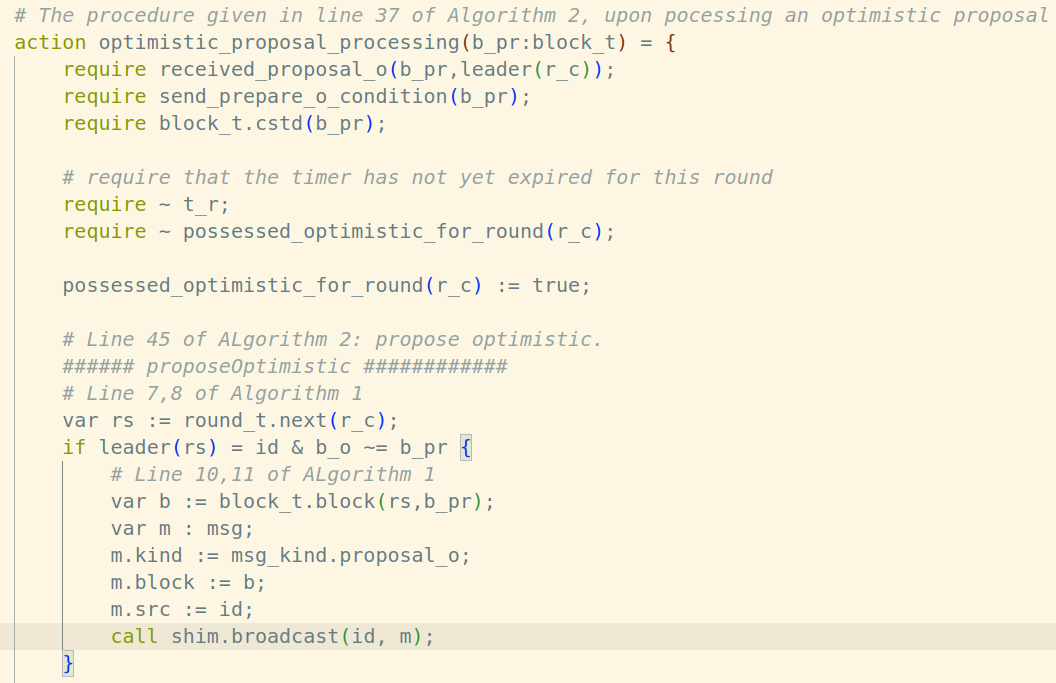
\includegraphics[scale=0.25]{OptimisticPropProc.png}
\end{frame}

\begin{frame}
    \frametitle{Artefacts of the project}
    \alert{quorum\textunderscore{}verification.ivy} - IVy shortcut
    for cryptographic checks of quorum certificates
    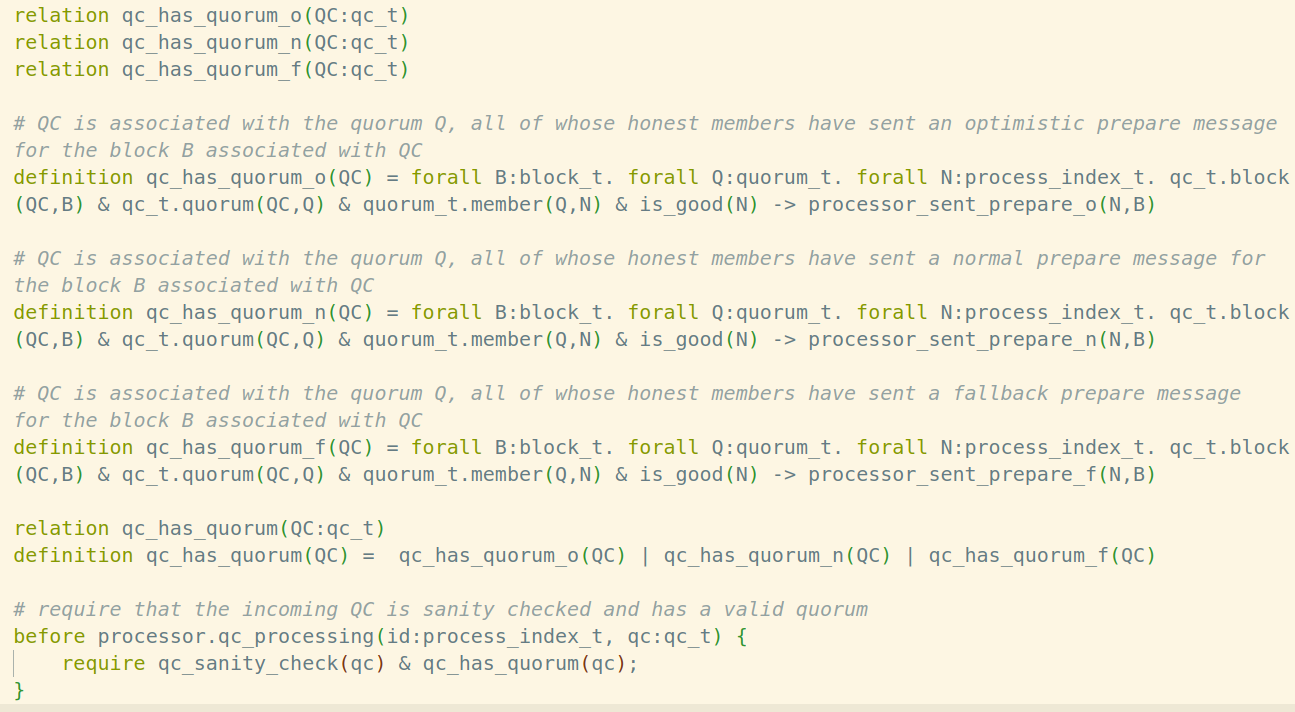
\includegraphics[scale=0.25]{QuorumDef.png}
\end{frame}

\begin{frame}
    \frametitle{Artefacts of the project}
    \alert{safety.ivy} - properties to be verified
    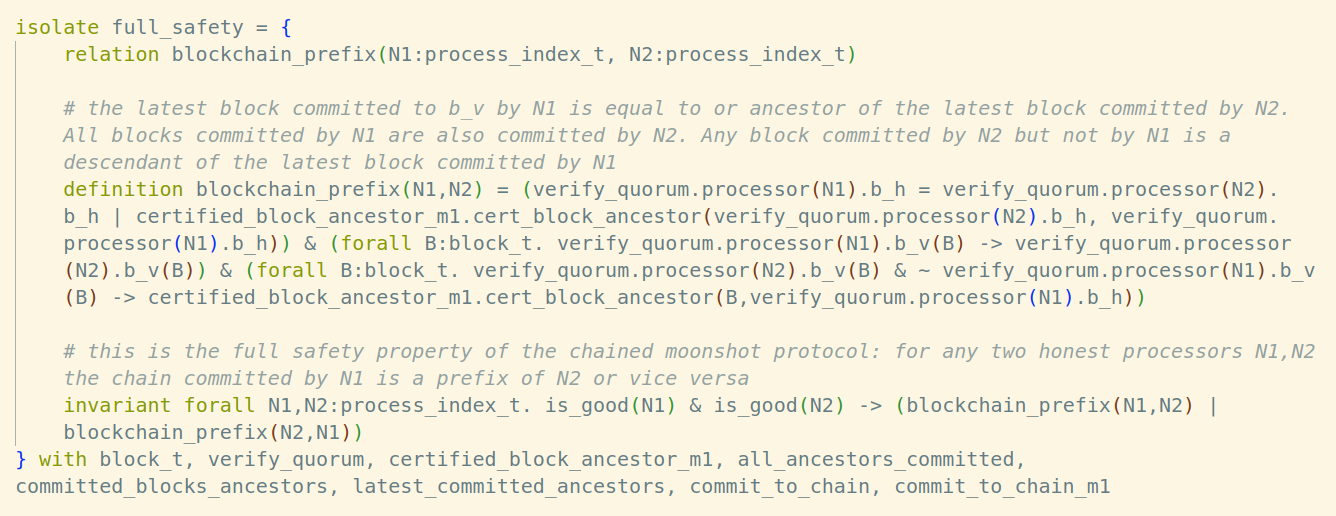
\includegraphics[scale=0.25]{FullSafety.png}
\end{frame}

\begin{frame}
    \frametitle{Byzantine nodes}
    They can send any kind of message to anybody, posing as any other
    Byzantine node
    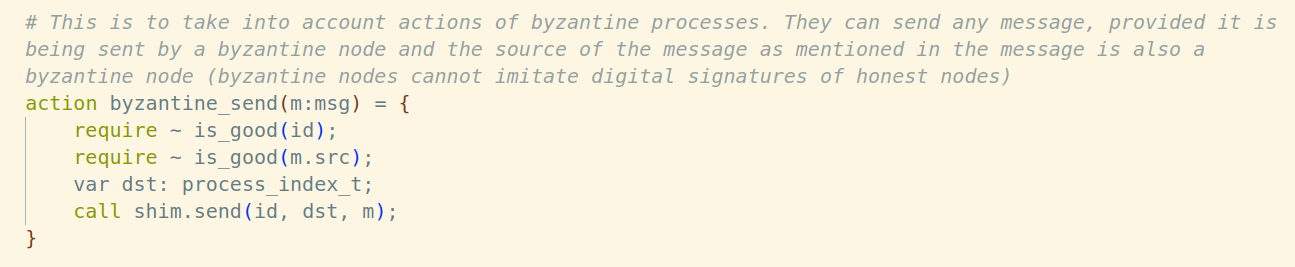
\includegraphics[scale=0.25]{ByzantineSendMsg.png}
    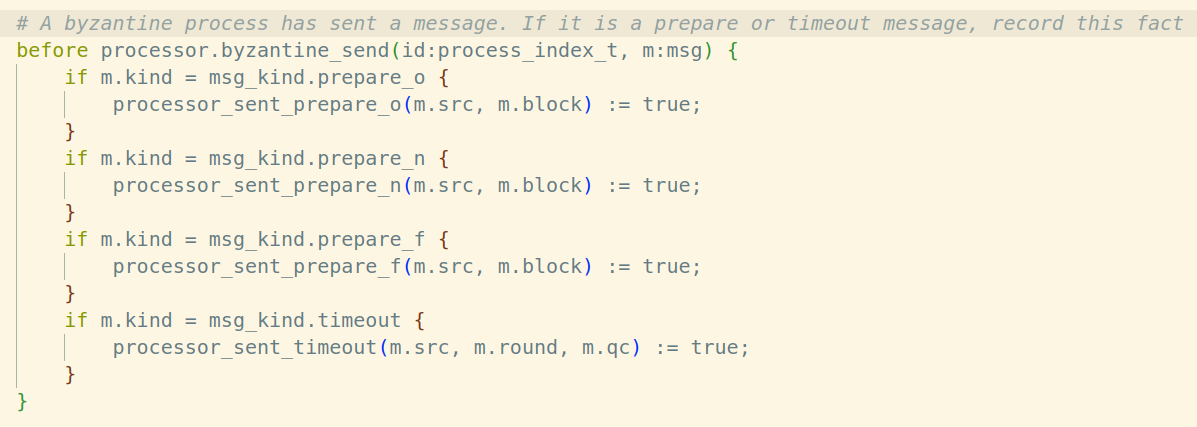
\includegraphics[scale=0.25]{RecordByzantineAction.png}
\end{frame}

\begin{frame}
    \frametitle{Every Minute Detail is Checked}
    Example - If an honest processor votes for a block B, B's parent
    Bp has a lesser round
    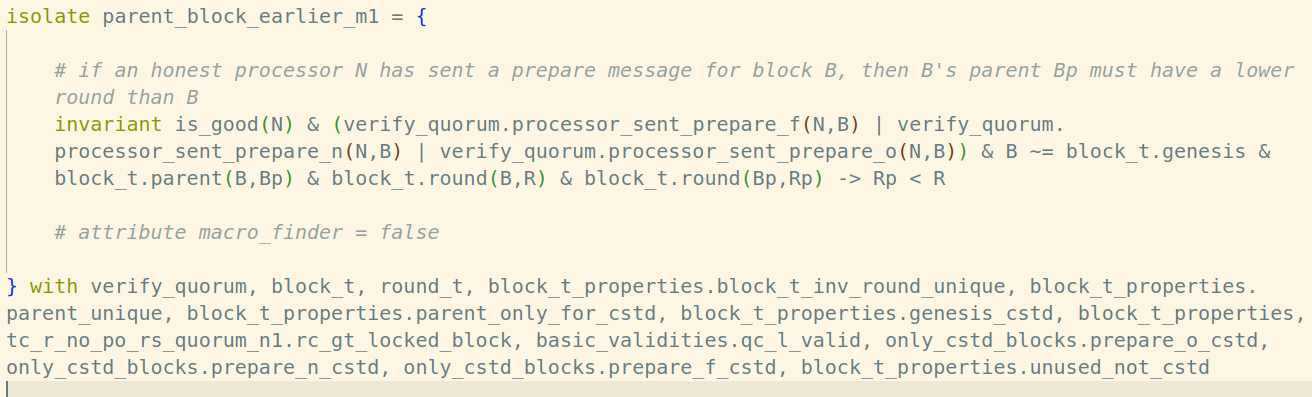
\includegraphics[scale=0.25]{ParentBlockEarlier.png}
    \pause
    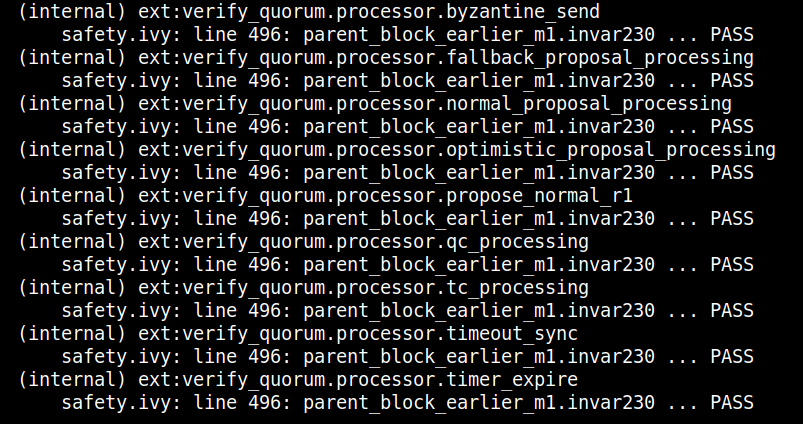
\includegraphics[scale=0.25]{ParentBlockEarlierPass.png}
\end{frame}

\begin{frame}
    \frametitle{Every Minute Detail is Checked}
    Depends on another property: while processing fallback proposals,
    all the QC's in the TC are processed first, so that the current
    round 
    r\textunderscore{}c is strictly greater
    than maxQC of the TC 
    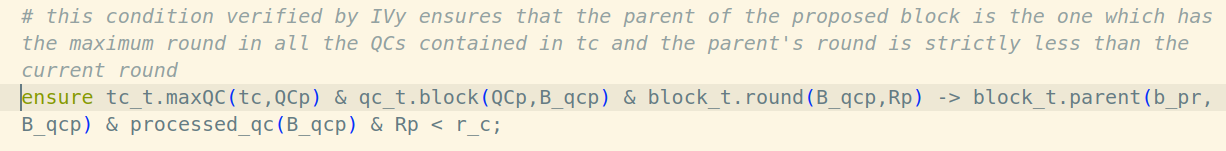
\includegraphics[scale=0.25]{RcGtMaxQC.png}
    \pause
    Suppose we omit the other property
    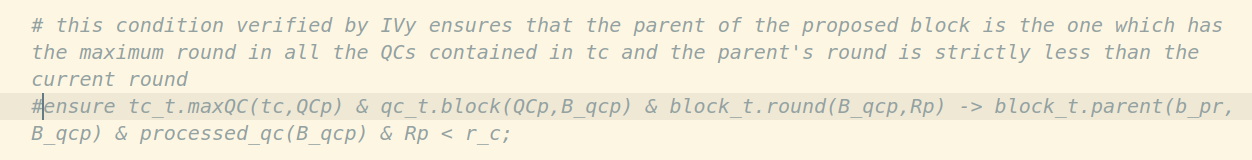
\includegraphics[scale=0.25]{RcGtMaxQCOmit.png}
    \pause
    IVy gives a counter example - block B of round 1 can have parent
    block Bp of round 2
    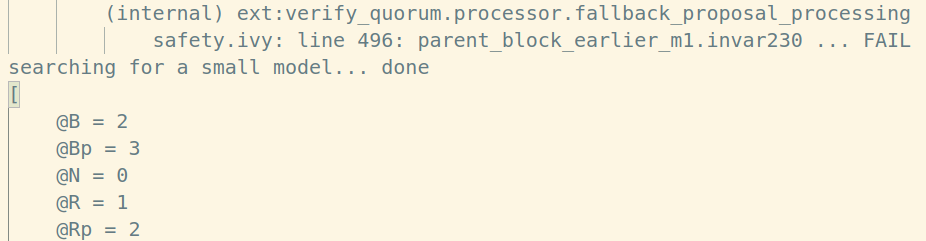
\includegraphics[scale=0.25]{ParentBlockEarlierViolated.png}
\end{frame}

\begin{frame}
    \frametitle{Structure of the safety proof}
    Follows the structure of the proof from Supra Research teams'
    paper

    Theorem 1 is the full safety, the last invariant in safety.ivy
    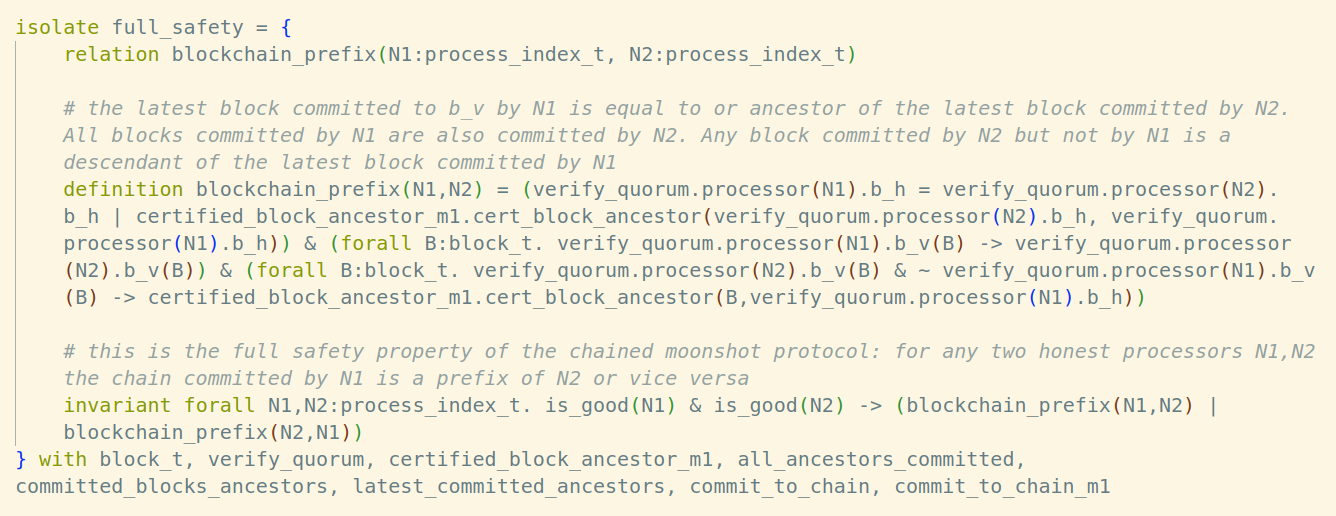
\includegraphics[scale=0.25]{FullSafety.png}
\end{frame}

\begin{frame}
    \frametitle{Structure of the safety proof}

    Depends on Corollary 4, called
    latest\textunderscore{}committed\textunderscore{}ancestors in
    safety.ivy
    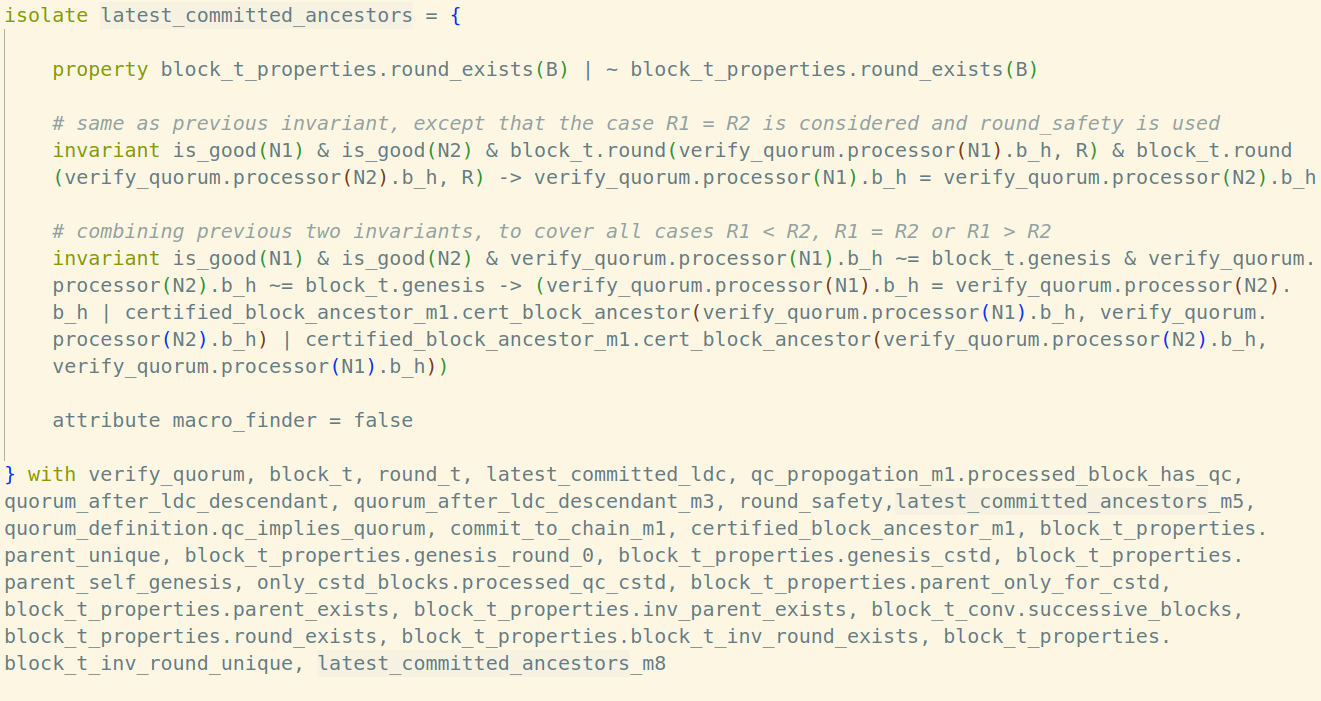
\includegraphics[scale=0.25]{Corollary4.png}

    Proving Corollary 4 is laborious, depends on many other properties
\end{frame}

\begin{frame}
    \frametitle{Structure of the safety proof}
    \begin{itemize}
        \item For proving one invariant, we may need to prove another
            one first \dots
            \pause
            \vfill
        \item Some invariant may be valid, but Z3 gets stuck, so we
            have to logically decompose it into smaller ones for Z3 to
            handle \dots
            \pause
            \vfill
        \item There are totally around 250 invariants that finally
            prove Theorem 1. All are manually written
            \pause
            \vfill
        \item Moonshot has a complicated pipelining mechanism to
            improve communication complexity. This is the first time a
            such a complicated protocol has been formally verified
    \end{itemize}
    \pause
    \vfill
    \begin{center}
        \Large{Thank You}
    \end{center}
\end{frame}
\end{document}
